\chapter{运动}

\section{运动的描述}

为了找出物体随时间而发生的各种变化所遵循的规律,我们必须\uwave{描述}这些变化,并用某种方式把它们记录下来。在物体中要观察的最简单的变化是物体的位置随时间的明显改变,我们把它称之为运动。让我们考虑一些固体吧,它们身上带有一个固定的可观测标记,这个我们后面会称之为点。我们将讨论这个小标记的运动(这个小标记可以是一辆汽车的散热器盖子,或一个下落的球的球心),并将试图描述它在运动以及如何运动这一事实。

这些例子看来似较平庸,但在描述其变化时,也有许多要小心对付之处。有些变化,例如,一朵缓慢漂移但迅速形成或迅速蒸发的云的漂移速率,或者一个女人思想上的变化,要描述它们就比描述在固体上一点的运动困难得多。我们不懂得分析思想上发生变化的简单方法,不过由于云可以用许多分子来表示或描述,或许在原则上我们能够通过描述云中所有个别分子的运动来描述云的运动。同样,或许思想上的变化甚至也与大脑内原子的变化有类似之处,但我们对此尚一无所知。

总而言之,这就是我们为什么要从点的运动开始研究的原因;也许我们应当把它们想像为原子,但在开始时粗糙一些可能更妥当。我们把它们简单地想像为某一类小的物体——所谓小,是指与运动的距离相比较而言。比如,在描述一辆开过一百公里的汽车的运动时,就不必区分汽车的前部和后部。的确,这里有一点差别,但粗略的看我们只讲“汽车”的运动,同样,我们选择的点不是绝对的点也丝毫没有关系;就我们现在的目的来说,没有必要极其精确。还有,在初次考察这个课题时,我们将不考虑世界的三维性。我们将只集中注意一个方向上的运动,就像在一条公路上行驶的汽车那样。当我们知道了如何描写一维运动后,就将回到三维中去。现在,你们会说:“这尽是一些琐碎的事。”确实如此。那么,我们怎样来描述这样的一维运动,比方说,汽车的运动呢?没有比这更简单的了。有许多可能的方式,下面是其中之一,为了确定不同时刻汽车的位置,我们测量它与起点的距离,并记下所有的观测。在表8.1中,$s$表示汽车离起点的距离,单位是英尺,$t$表示时间,单位是分。表中的第一行表示零距离和零时间——即汽车尚未出发。一分钟后,出发并开过了1200英尺。在两分钟内,它开得更远——注意汽车在第二分钟开过了更大的距离——并且加速前进;但在第三和第四分钟或者甚至一直到第五分钟之间发生了一些情况——也许是遇到红灯停了下来?然后它再次加速,在第六分钟末开过13000英尺,在第七分钟末开过18000英尺,在第八分钟开过23500英尺,在第九分钟它只前进到24000英尺,因为在最后一分钟它被警察拦住了。

\label{tab:表8.1}
\noindent
\begin{minipage}{\textwidth}
\begin{minipage}{0.3\textwidth}
\begin{table}[H]
    \centering
    \medskip 
    \scalebox{0.82}{
    \begin{tabular}{@{}ll@{}}
    \toprule
    $t$(分) & $s$(英尺)  \\ \midrule
    0 & 0     \\
    1 & 1200  \\
    2 & 4000  \\
    3 & 9000  \\
    4 & 9500  \\
    5 & 9600  \\
    6 & 13000 \\
    7 & 18000 \\
    8 & 23500 \\
    9 & 24000 
    \\ \bottomrule
    \end{tabular}
    }
    \caption*{表 8.1}
\end{table}
\end{minipage}\hfill
\begin{minipage}{0.7\textwidth}
\begin{figure}[H]
    \centering
    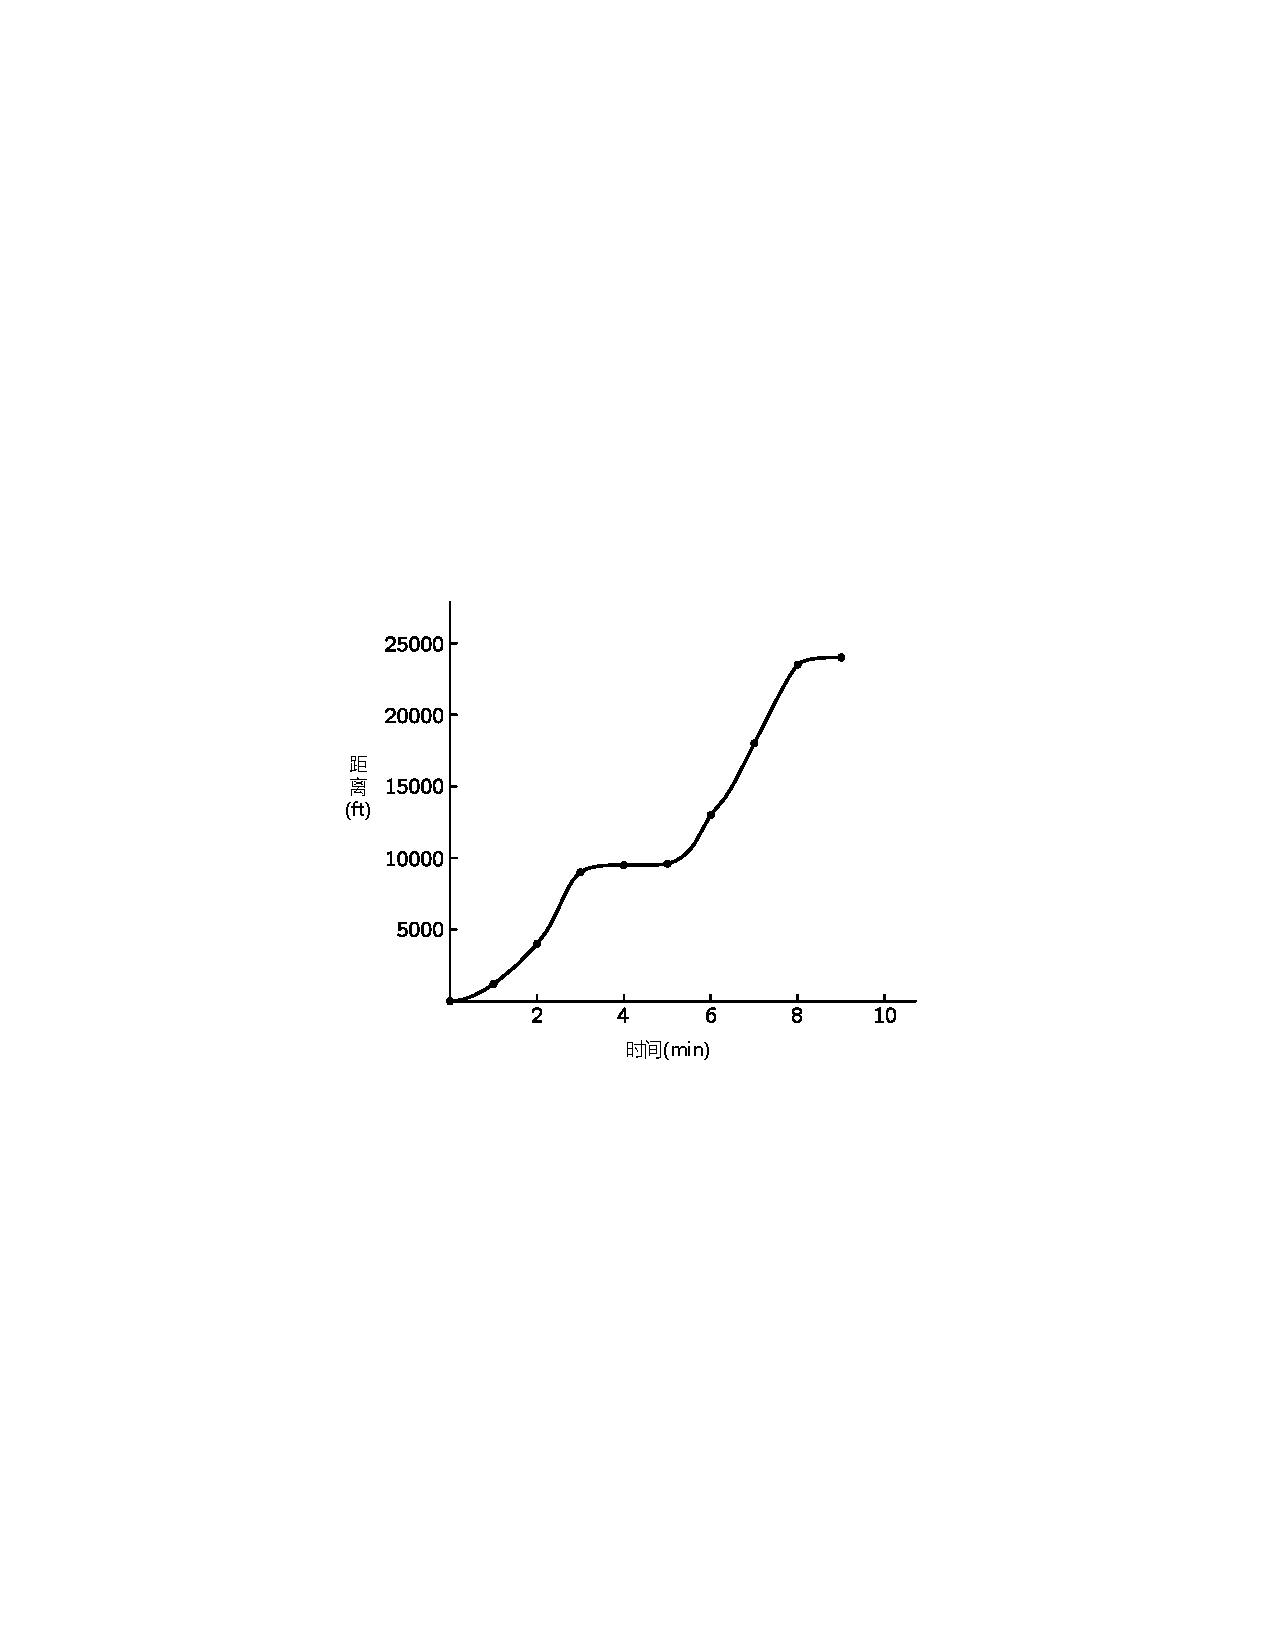
\includegraphics[width=0.75\linewidth ,totalheight=0.8\textheight , keepaspectratio]{Chapter8/汽车的距离-时间曲线}
    \caption{汽车的距离-时间曲线}
    \label{figure:汽车的距离-时间曲线}
\end{figure}
\end{minipage} 
\end{minipage} 


\label{tab:表8.2}
\noindent
\begin{minipage}{\textwidth}
\begin{minipage}{0.3\textwidth}
\begin{table}[H]
    \centering
    \medskip 
    \scalebox{0.9}{
    \begin{tabular}{@{}ll@{}}
    \toprule
    $t$(分) & $s$(英尺)  \\ \midrule
    0 & 0     \\
    1 & 16  \\
    2 & 64  \\
    3 & 144  \\
    4 & 256  \\
    5 & 400  \\
    6 & 576 
    \\ \bottomrule
    \end{tabular}
    }
    \caption*{表 8.2}
\end{table}
\end{minipage}\hfill
    \begin{minipage}{0.7\textwidth}
        \begin{figure}[H]
            \centering
            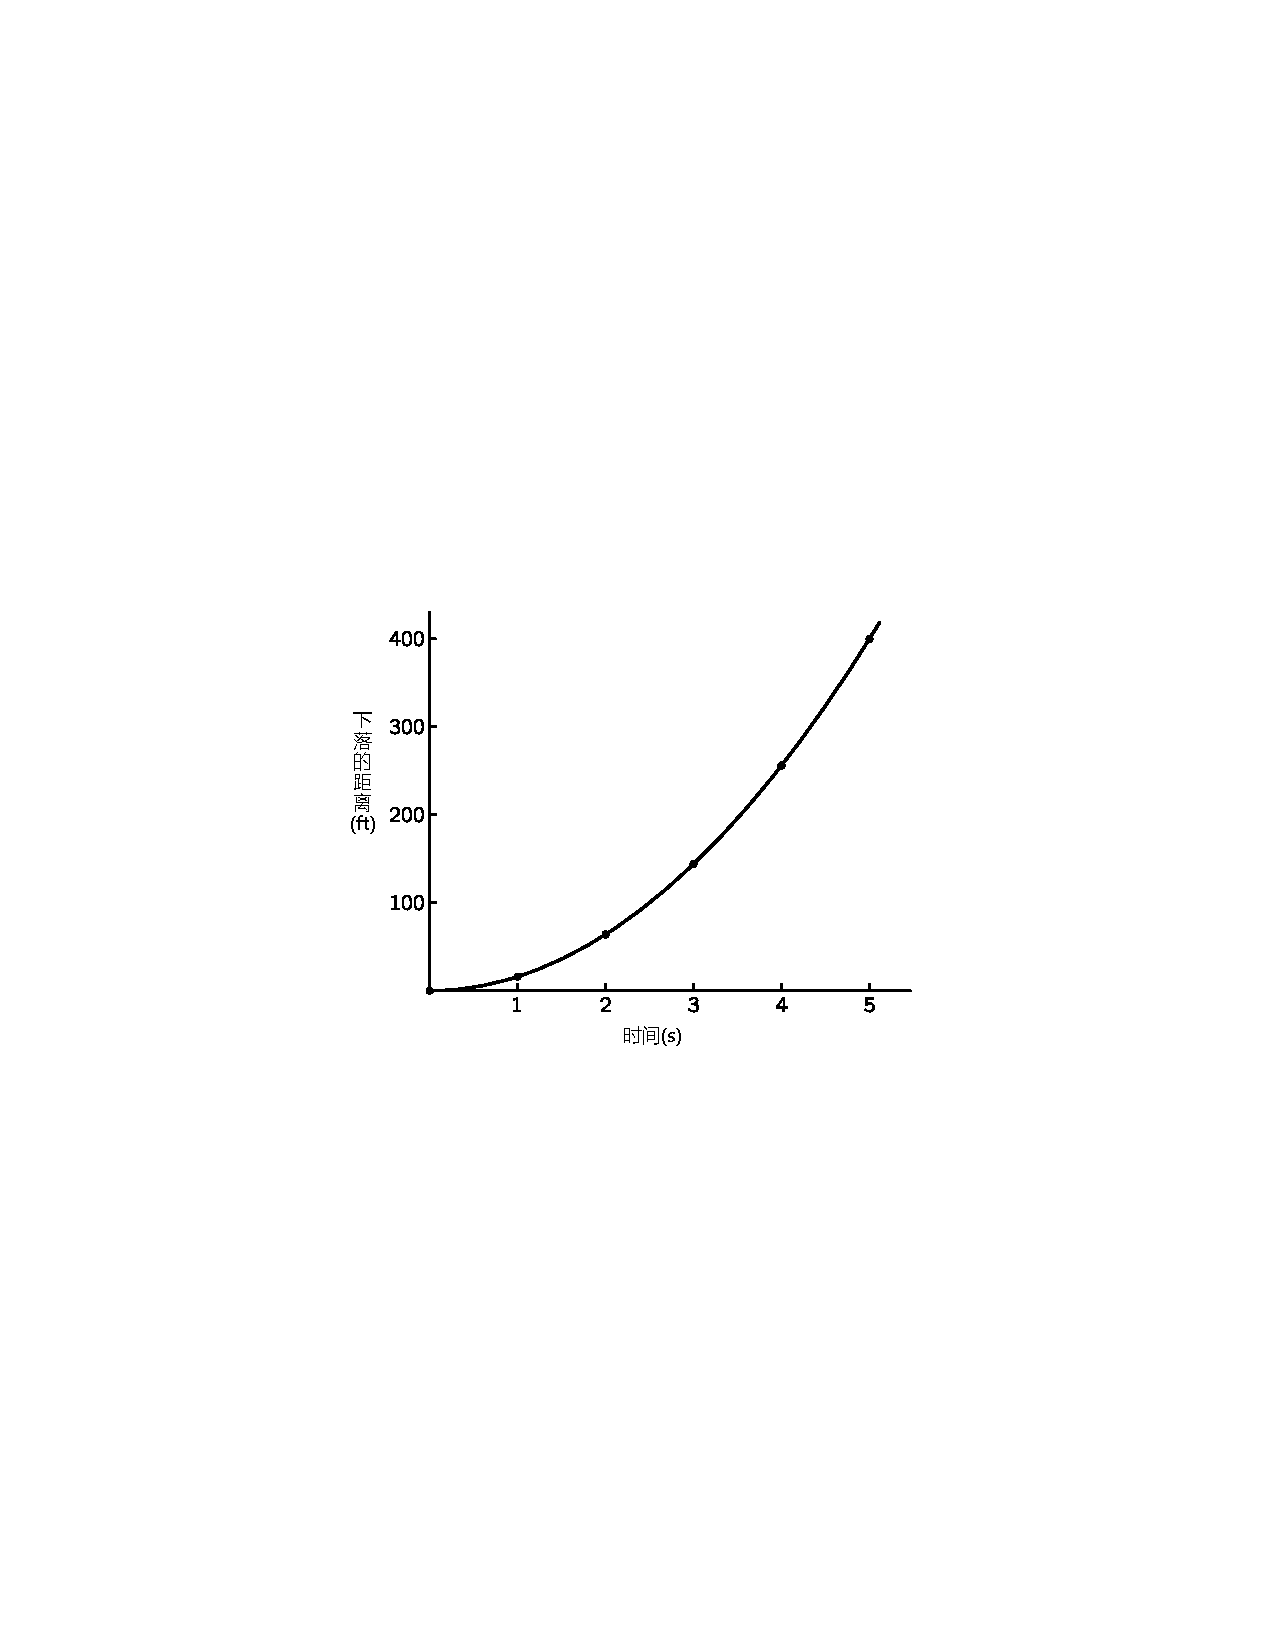
\includegraphics[width=0.75\linewidth ,totalheight=0.8\textheight , keepaspectratio]{Chapter8/落体的距离-时间曲线}
            \caption{落体的距离-时间曲线}
            \label{figure:落体的距离-时间曲线}
        \end{figure}
    \end{minipage} 
\end{minipage} 

这就是一种描写运动的方式,另一种方式是借助于图画。如果我们以横轴表示时间,纵轴表示距离,就得到如图8.1那样的一条曲线。当时间增加时,距离也增加,开始很慢,然后很快,在四分钟前后又很慢,以后几分钟内又再加快,最后在九分钟时,看来像停止增加了。这些情况不用表也能从图上观察到。显然,为了描述完全起见,人们还知道,在那些半分钟的标记处,汽车开到了那里。但是我们假定这个曲线图可以这样来解释,在所有的中间时刻汽车都具有某个位置。

汽车的运动是复杂的,另外我们举一个遵循简单的法则以简单的方式运动的例子,比如说一个下落的小球。表8.2列出了落体的时间(以秒为单位)和距离(以英尺为单位)。在零秒时,小球从零英尺开始下落,在第一秒末落下16英尺,在第二秒末落下64英尺,在第三秒末落下144英尺,等等。如果将表上的数字作图,就得到图8.2所示的一条漂亮的抛物线。这条曲线的公式可以写成
\begin{equation}
\label{Eq:I:8:1}
s=16t^2.
\end{equation}
这个公式使我们可以计算小球在任何时刻的距离。你们或许会说,对第一个曲线图也应当有个公式。实际上,人们也可以抽象地把这样一个公式写成
\begin{equation}
\label{Eq:I:8:2}
s=f(t),
\end{equation}
它表示$s$是某个依赖于$t$的量,或用数学术语来说,$s$是$t$的函数。由于我们不知道这个函数是什么,因此无法以确定的代数形式写下来。

现在我们已经看到了两个用非常简单的思想就能适当地描述的运动的例子——没有什么难以捉摸之处。然而,难以捉摸之处还是有的,\uwave{有几处}。首先,\uwave{时间}和\uwave{空间}究竟意味着什么?结果表明,这些深刻的哲学问题在物理学上必须十分小心地加以分析,而着并不是容易做到的。相对论表明我们关于空间和时间的观念并不如人们乍一看来可以想像的那么简单。然而,就我们当前的目的而论,对我们在开始时所要求的精确度来说,我们毋需十分小心地去精确定义事物。或许你们要说:“这很糟糕,我听说过在科学上我们必须静确定定义每一件事。”我们不可能精确地定义\uwave{任何事物}!如果强求如此,只会使我们陷入像某些哲学家那样的思想僵化,他们面对面坐着,一个对另一个说:“你不知道你在讲些什么!”第二个说:“你所谓的‘\uwave{知道}’是什么意思呢?你所谓的‘\uwave{讲}’是什么意思呢?你所谓的‘\uwave{你}’又是什么意思呢?如此之类。”为了能够进行建设性的讨论,我们必须一致赞同我们所谈论的大致是同一件事。你们对于时间的了解已能满足我们目前的需要,但必须记住,还有一些微妙和难以捉摸的事情需要讨论,我们将在以后进行。

前面所涉及的另一个难以捉摸之处是能够设想我们正在观察的动点总是位于某处(当然,当我们注视它时,它在那里,但当我们看别处时,它可能不在那儿了。)现在知道,在原子的运动中,这个观念也是错误的,我们不可能在一个原子上找到一个标记并观察它的运动。这种微妙的情况我们将在量子力学中去仔细讨论,但是在引进复杂性之前,我们将首先了解一下这些问题是什么,\uwave{然后}才能较好地按照这个题材的更现代的知识进行修正。因此,关于时间和空间,我们将采用一种简单的观点。我们大致知道这些概念是怎么一回事,而那些驾驶汽车的人则知道速率指的是什么。

\section{速率}

尽管我们知道大概“速率”的意思,但这里还是有一些比较深的奥妙;要知道博学的希腊人也从未能恰当地描述牵涉到速度的问题。这奥妙就在于准确地理解到底什么才是“速率”,希腊人对这个问题感到很困惑,这是因为要发现一个新的数学分支才能解决这个问题,而这是超越于希腊人、阿拉伯人与巴比伦人固有的几何学与代数学之外的 。作为这个难点的一个例证,试用纯代数方法来解这样一个问题:一个气球正在膨胀,它的体积以每秒100厘米的比率增加;当气球体积为1000$\text{厘米}^3$时,气球半径增加的速率是多少?希腊人多少有点被这样的问题弄糊涂了。当然,这是被某些思想混乱的人所促成的。为了指出在某一时刻有关速度方面的推理上存在着困难,芝诺(Zeno)提出了一大堆佯谬,我们将举其中的一个来说明他的关于思考运动时存在着明显困难的论点。“请听这样的论点”,他说:“阿基利斯(Achilles)比乌龟跑得快10倍,但他却永远抓不住乌龟。因为,假定他们开始赛跑时,乌龟在阿基利斯前面100米,那么当阿基利斯跑了100米而到达乌龟原来所在的地方时,乌龟已经以他的快慢的$1/10$前进了10米。现在,阿基利斯又得跑另一个10米以便赶上乌龟,但在到达跑步的终点时,他发现乌龟仍在他前面1米;当他再跑1米时,他又发现乌龟依然在他前面10厘米,如此下去,\uwave{直至无穷}。因此,在任何时刻乌龟总是在阿基利斯前面,阿基利斯永远追不上乌龟。”这段论证错在那里?它错在认为一段有限的时间可以被分为无限多的小份,正如一条线段不断地一分为二分成无限多的小段一样。因此,虽然(在论证中)直到阿基利斯追上乌龟可以分成无穷多步,但是并不意味着是无穷无尽的\uwave{时间}。从这个例子我们可以看到,在有关速率的理解上,还是有所玄机的。

为了以更为清楚的方式来领会这所谓的玄机,我讲一个你们肯定听到过的笑话。坐在汽车里面的一位太太在某个地点被警察拦住了,警察走过来对她说:“太太,你刚才的车速是每小时60英里!”她反驳道:“先生,这是不可能的,我刚才只开了七分钟。这正是天大的笑话!我开车还没有到一个小时,怎么可能每小时走60英里呢?”假如你是警察的话你该如何回答她呢?当然,如果你真是那个警察,那就没有什么疑难之处;很简单,你会说:“对审判官讲去!”但是,假若我们没有这条退路,并且更公正和理智地对待这个问题,企图向这位太太解释所谓她的车速达每小时60英里的说法是什么意思,那么我们的含义\uwave{究竟}是什么呢?我们可以说:“太太,我们的意思是:如果你继续像现在这样开车,在下一个小时里你将开过60英里。”她会答道:“嗯,我的脚已经离开油门,汽车已慢了下来,所以如果我继续这样开下去,不会超过60英里的。”或者,我们考虑一个自由下落的小球,如果这个小球保持它正在进行的运动方式的话,我们想要知道它在第三秒时的速率有多大。这意味着什么呢?是继续\uwave{加速},落得更快吗?不,应该是继续以同样的\uwave{速度}运动。但这正是我们试图加以定义的东西!因为如果小球保持它现在正在进行的方式运动,那么它在以后就将继续保持这种方式运动。于是我们就需要更好地定义速度,究竟是什么必须保持一样呢?这位太太也可以这样来辩护:“如果我再继续保持现在的开车方式,那么过了一个小时后,我就会撞到街道尽头的墙上了!”看来要说清楚我们的意思并不那么容易。

许多物理学家认为测量是唯一定义任何事物的方式。那么,显然,我们应当使用测量速率的仪器——速度计,并说:“!太太,你的速度计的读数指到60。”可是她说:“我的速度计坏了,根本不能读数。”这是否表示汽车停着不动呢?我们相信,在我们造出速度计之前,就存在某种要测量的东西。只有这样,我们才可以说:“速度计走得不准,”或“速度计坏了。”如果速度脱离了速度计就没有意义了,那这么讲就毫无道理了。所以,显然在我们的头脑中存在着一种与速度计无关的概念,速度计只是用来使这个概念计量化罢了。所以,还是让我们来看看是否能得到比这个想法更好的定义。我们可以说:“嗯!固然在你的车子开了一个小时以前,你就会撞到墙上,但是如果你开了一秒钟,你就会通过88英尺的距离。太太\footnote{这一定是苏格拉底的太太。。},你刚才的车速正是每秒88英尺,如果继续下去,下一秒也将开过88英尺,而那堵墙离这还远着呢。”她就说:“对,但是,没有一条法律禁止每秒88英尺的车速!只有一条禁止每小时开60英里的法律。”“不过”我们反驳道:“这是同一件事。”如果这\uwave{确实是}同一件事,那就毋需赘言每秒88英尺了。事实上,自由落体甚至连一秒钟也不可能保持同样的运动方式,因为它的快慢在变化着,我们必须设法来定义速率了。

现在看来,我们已经走上正规了,似乎可以这样说:如果那位太太在另一个$1/1000$小时内继续这样行驶,她将开过60英里的一千分之一。换句话说,她毋需继续开足一小时,主要在于,\uwave{在某一瞬间}她正以这个速率开车。现在我们的意思是,只要她再多开一点点时间,那么汽车所通过的外加距离就和一辆以每小时60英里的\uwave{稳定}速率开动的汽车相同。也许每秒88英尺的观念是正确的,我们看看她在最后一秒钟开了多远,再除以88英尺,如果结果是1,那么速率就是每小时60英里。换句话说,可以这样来求出速率:我们问在一个很短的时间内物体走过多远?把这一段距离除以时间就得到速率。但是应当把这段时间取得尽可能短,越短越好,因为在这段时间内有可能发生某种变化。假如我们将落体的时间取为一小时,这个概念就荒唐了。但若取为一秒,对汽车来说结果就相当好,因为在这段时间内,汽车的快慢没有很大变化,但对落体来说就不行了。所以为了要得到越来越精确的速率,我们应当把时间间隔取得越来越小。我们应当做的是取百分之一秒,并且用百分之一秒去除通过的距离,结果给出每秒的距离,这就是我们所谓的速度。因此我们可以用这个方式去定义它。这是为那位太太给出的成功的答案,或者更确切地说,它就是我们将要采用的定义。

上述定义包括了一个新的概念,这是一个希腊人不曾以普遍形式采用过的概念。这个概念就是取无穷小距离及相应的\uwave{无穷小时间},求出它们的比值,并观察我们所取的时间越来越小时,那个比值将发生一些什么情况。换句话说,当时间越取越小,\uwave{以至无穷小}时,取所通过的距离除以所需的时间的极限。这个概念分别由牛顿和莱布尼兹发现,它开创了称为\uwave{微分学}的新的数学分支。微积分的发现是为了描述运动,而它的第一个应用就是给“每小时开60英里”作什么解释下一个定义。

让我们试试看把速度定义得更好一些,假设在一个短时间$\epsilon$内,汽车或其他物体通过一段短距离$x$,则速度$v$定义为
\begin{equation*}
v=x/\epsilon,
\end{equation*}
这是一个近似,当$\epsilon$取得越来越小,近似程度就越来越好。如果想用一个数学表达式,我们可以说速度等于在表达式$x/\epsilon$中,当$\epsilon$越来越小时的极限,即
\begin{equation}
\label{Eq:I:8:3}
v=\lim_{\epsilon\to0}\frac{x}{\epsilon}.
\end{equation}
我们不可能对汽车里面的那位太太做同样的事情,因为那张表是不完全的。我们只知道她在各个间隔为一分钟的时刻的位置,我们能得到在第七分钟那段时间她开车的速率是5000英尺/分这一大致概念,但无法知道,在正好是第七分钟那个时刻,她是否已经加速运动,是否在第六分钟开始时速率是4900英尺/分,而现在是5100英尺/分,或者其他情况,因为我们没有获知其间的精确细节。因此只有以无穷个数据来完成这张表,我们才能真正从这样一张表来计算速度。另一方面,如果我们有一个完整的数学公式,就像在落体的情况下(式\ref{Eq:I:8:1})那样,就有可能计算速度,因为我们可以计算出在无论任何时刻的位置。

作为例子,我们来决定落体在5秒那个特定时刻的速度。一个方法是由表\ref{tab:表8.2}中看出它在第5秒内的情况,它走了$400-256=144$英尺,因此它正以144英尺/秒下落;可是这是错误的,因为速率正在发生变化,在这段时间间隔内,平均来说是144英尺/秒,但这个球在加速,并且实际上走得比144英尺/秒要快。我们希望弄清楚它的速度究竟有多快。在这个过程中涉及的方法如下:我们知道在5秒时球在那里。在5.1秒时,它总共走过的距离是$16(5.1)^2=416.16$英尺(见式\ref{Eq:I:8:1})。在第5秒时它已下落400英尺,在最后的$1/10$秒内它下落了$416.16-400=16.16$英尺。由于在0.1秒中通过16.16英尺与161.6英尺/秒是同一回事,这差不多就是速率,但还不完全正确。它究竟是5秒、5.1秒抑或是二者当中的5.05秒时的速度呢?或者说,\uwave{是}什么时刻的速度?别管它——现在的问题是要求出在5秒时的速率,而我们还没有得到精确的答案;我们必须做得更好。于是,我们比5秒多取千分之一秒,即5.001秒,再计算这时总下落的距离
\begin{equation*}
s=16(5.001)^2=16(25.010001)=400.160016 \,\textrm{英尺}.
\end{equation*}
在最后0.001秒内球落下了0.160016英尺,如以0.001秒除之,就得到速率为160.016英尺/秒。这个值更为接近,而且十分接近,但它\uwave{仍不精确}。为了找出准确的速率,我们必须做什么是很明显的。为了完成这个数学过程,我们把问题提得略为抽象一点;要求出在某一特定时刻$t_0$时的速度,在上面的问题中,$t_0$就是5秒。现在在$t_0$时刻的距离,我们称为$s_0$是$16t_0^2$,或在这个情况下是400英尺。为了求出速度,我们问:“现在$t_0+\textrm{(一点点)}$,即$t_0+s$时物体在何处?”新位置是$16(t_0+\epsilon)^2=16t_0^2+32t_0\epsilon+16\epsilon^2$,于是它比以前走得更远了,因为以前它只是$16t_0^2$。这段距离我们称为$s_0+\textrm{(多一点点)}$或$s_0+x$(如果$x$是附加的一点点距离)。现在如果从在($t_0+\epsilon$)时刻的距离中减去在$t_0$时刻的距离,我们就得出$x$,即附加的距离,为$x=32t_0\cdot\epsilon+16\epsilon^2$。我们对速度的第一次近似是
\begin{equation}
\label{Eq:I:8:4}
v=\frac{x}{\epsilon}=32t_0+16\epsilon.
\end{equation}
真正的速度是当$\epsilon$变得趋于0那么小时的比值$x/\epsilon$。换句话说,在做出比值后,我们取当$\epsilon$越来越小,即趋于0时的极限。式(\ref{Eq:I:8:4})化为
\begin{equation*}
v\,(\textrm{在时刻$t_0$})=32t_0.
\end{equation*}
在我们的问题中$t_0=5$秒,故答案是$v=32\times5=160$英尺/秒。在前面,我们曾相继取$\epsilon=0.1$及$0.001$秒,所得到的$v$值比这稍大一点,但现在我们看到,实际速度正好是160英尺/秒。




\section{速率作为导数}
我们刚刚采用的步骤在数学上是经常要作的,因此为了方便起见,对量$\epsilon$和$x$规定了特殊的符号。在这一符号中,上面所用的$\epsilon$改为$\Delta t$,$x$改为$\Delta s$。$\Delta t$表示“额外的一点$t$”,并暗指它能变得更小。前缀$\Delta$不是一个常数,正如$\sin \theta$不是$\text{s}\cdot\text{i}\cdot\text{n}\cdot\theta$一样,它仅仅定义了一个时间增量,并使我们想起了它所具有的特性。$\Delta s$对距离$s$有类似的含义。因为$\Delta$不是一个因子,因此在比值$\Delta s/\Delta t$中不能消去而得出$s/t$,正如比值$\sin\theta/\sin2\theta$不能消去成为$1/2$一样。在这种符号下,速度等于当$\Delta t$变得越来越小时$\Delta s/\Delta t$的极限,即
\begin{equation}
\label{Eq:I:8:5}
v=\lim_{\Delta t\to0}\frac{\Delta s}{\Delta t}.
\end{equation}
实际上这和我们前面使用$\epsilon$与$x$的表达式(\ref{Eq:I:8:3})相同,但它的好处是表示某种东西在变化着,并且记录了什么东西正在发生变化。

顺便提一下,作为一个好的近似,我们还得出另一条定律:一个动点距离的变化是速度乘上时间间隔,或$\Delta s=v\,\Delta t$。这个说法仅当速度在这个时间间隔内不变时才正确,而这个条件又只是在$\Delta t$趋于0的极限情况下才成立。物理学家喜欢把它写为$ds=v\,dt$,因为按他们的意思$dt$是非常小的。根据这样的理解,这个表达式作为一个非常接近的近似是成立的。如果$\Delta t$太长,速度在这段间隔内可能发生变化,因而这个近似就欠佳了。对趋于0的时间$dt$,$ds=v\,dt$严格成立。用这种符号我们可将式(\ref{Eq:I:8:5})写为
\begin{equation*}
v=\lim_{\Delta t\to0}\frac{\Delta s}{\Delta t}=\frac{ds}{dt}.
\end{equation*}

我们在上面得到的量$ds/dt$叫做“$s$对于$t$的导数”(这个称呼有助于记下发生变化的过程),而求出它的复杂过程就称为求导,或求微商。单独出现的$ds$和$dt$叫做微分。为了让你们熟悉这些词,我们说我们已经找到函数$16t^2$的导数,或者$16t^2$对于$t$的导数是 $32t$。当我们习惯这些词之后,这些概念就更容易理解了。作为练习,让我们来求一个更复杂的函数的导数。我们将考虑公式$s=At^3+Bt+C$,它可以描述一点的运动。字母$A$,$B$,$C$表示常数,就像在常见的二次方程一般形式中一样\footnote{此处暗指$y=Ax^2+Bx+C$这样的形式。}。从这个运动公式出发,我们希望求出在任何时刻的速度。为了以比较巧妙的方式求得它,我们把$t$改为$t+\Delta t$,并注意$s$将随之变为$s+\textrm{某个}\Delta s$;然后我们求出用$\Delta t$来表示的$\Delta s$。这就是说
\begin{align*}
s+\Delta s&=A(t+\Delta t)^3+B(t+\Delta t)+C\\[1ex]
&=At^3+Bt+C+3At^2\,\Delta t+B\,\Delta t+3At(\Delta t)^2+
A(\Delta t)^3,
\end{align*}
但由于
\begin{equation*}
s=At^3+Bt+C,
\end{equation*}
因而
\begin{equation*}
\Delta s=3At^2\,\Delta t+B\,\Delta t+3At(\Delta t)^2+A(\Delta t)^3.
\end{equation*}
但是我们想要的不是$\Delta s$,而是$\Delta s$除以$\Delta t$。将上述等式除以$\Delta t$,得
\begin{equation*}
\frac{\Delta s}{\Delta t}=3At^2+B+3At(\Delta t)+A(\Delta t)^2.
\end{equation*}
当$\Delta t$趋于0时,$\Delta s/\Delta t$的极限是$ds/dt$,并等于
\begin{equation*}
\frac{s}{t}=3At^2+B.
\end{equation*}
这就是微积分的基本运算过程,对函数求微商。这个过程甚至可以比上面所讲的更简单一些。当观察到这些展开式中含有$\Delta t$的平方项、立方项或任何更高次幂时,这种项可以马上去掉,因为取极限时它们变为0。在稍微练习一下后,这个过程就显得方便了,因为我们知道把什么去掉。为了求出不同类型的函数的微商,有许多规则或公式。这些规则或公式可以记住,也可以在表中找到。表8.3就是一张简表。
\begin{table}[H]
\renewcommand{\arraystretch}{1.5}
\centering
\label{tab:求导简表}
\caption{求~导~简~表 \\{\footnotesize $s, u, v, w$是$t$的任意函数;$a, b, c, n$是任意常数}}
\medskip 
\begin{tabular}{@{}ll@{}}
\toprule
函数 & 导数  \\ \midrule
$s=t^n$  & $\frac{ds}{dt}=nt^{n-1}$  \\
$s=cu$  & $\frac{ds}{dt}=c\,\frac{du}{dt}$ \\
$s=u+v+w+\dotsb\qquad $ & $ \frac{ds}{dt}=\frac{du}{dt}+\frac{dv}{dt}+\frac{dw}{dt}+\dotsb$  \\
$s=c$ & $\frac{ds}{dt}=0 $ \\
$s=u^av^bw^c\dotsm$ & $\frac{ds}{dt}=s\biggl(\frac{a}{u}\,\frac{du}{dt}+
\frac{b}{v}\,\frac{dv}{dt}+\frac{c}{w}\,\frac{dw}{dt}+\dotsb\biggr)$
 \\ \bottomrule
\end{tabular}
\end{table}




\section{距离作为积分}
现在我们讨论相反的问题。假定我们不是有一张距离的表,而是有一张从零开始,在不同时刻的速率表。对一个下落的球,它的速率和时间如表8.4所示。
\begin{table}[H]
\centering
\caption{自由下落小球的速度}
\label{tab:8.2}
\medskip 
\begin{tabular}{@{}ll@{}}
\toprule
$t$(秒) & $v$(英尺/秒)  \\ \midrule
0  & 0  \\
1  & 32 \\
2  & 64 \\
3  & 96 \\
4  & 128 
 \\ \bottomrule
\end{tabular}
\end{table}

每分钟或每半分钟记录一次速度计的读数也可以对汽车的速度作出类似的表。假如我们知道汽车在任何时刻开得多快,我们能确定它开了多远吗?这个问题恰好与上面所解决的问题相反,即给出速度而要求出距离。如果我们知道了速度,我们怎样找出距离呢?假定汽车的速度不是常数,而那位太太在某个时刻每小时开60英里,然后慢下来,再加快,等等,我们如何来确定汽车走了多远呢?这很容易。我们使用同样的概念,并将距离表示成许多个无穷小量之和。我们说:“在第一秒钟汽车的速度是如此如此,并由公式$\Delta s=v\,\Delta t$,计算出它以这个速度在第一秒内走了多远。”而在下一秒钟内它的速度近似相同,但略有差别。我们可以用新的速率乘以时间来计算出这下一秒它走了多远。对每一秒我们都同样处理,知道路程的终点为止。现在我们就求得了一系列小距离,总距离就是这些小距离之和。也就是距离是速率乘以时间的和,或$s=\sum v\,\Delta t$,这里希腊字母$\sum$(sigma)表示累加。说得更加确切一些,距离是在某一确定时刻,比方在第$i$个时刻的速度乘以$\Delta t$以后的和。
\begin{equation}
\label{Eq:I:8:6}
s=\sum_iv(t_i)\,\Delta t.
\end{equation}
这里关于时间的规则是$t_{i+1}=t_i+\Delta t$。然而,我们用这个方法得到的距离是不准确的,因为在时间间隔$\Delta t$内速度已发生变化。假定我们将时间取得足够短,和就是精确的了,于是我们将时间取得越来越小,直到获得所需要的精确度为止。真正的$s$是
\begin{equation}
\label{Eq:I:8:7}
s=\lim_{\Delta t\to0}\sum_iv(t_i)\,\Delta t.
\end{equation}
类似于微分符号,数学家们对这个极限也规定了一个符号。式(\ref{Eq:I:8:7})中的$\Delta$变为$d$,以提醒我们时间是尽可能地短,于是速度就是在时刻$t$的$v$,累加则写成拉长了的“s”——$\int$[从拉丁文summa(和)而来],遗憾的是现在没有正式名称,只是称为积分符号。所以我们这样写到
\begin{equation}
\label{Eq:I:8:8}
s=\int v(t)\,dt.
\end{equation}
将所有这些项加起来的过程称为积分,它和微分互为相反的过程。这个积分公式的导数就是$v$,所以一个运算符号($d$)就消除了另一个运算符号($\int$)。人们可以把求微商的公式反过来,以得到一些积分公式,因为它们彼此正好是相反的运算。于是,对所有类型的函数求微分,人们就可以得出他们的积分表。对每个微分公式,如果我们把它倒过来,就得到一个积分公式。

每个函数可以用解析的方法微分, 即这个过程能用代数方法来进行,并得出某个有定义的函数。但是,对随意给定的积分却不能用简单的方式写出解析解来。不过你们可以计算它,比如,上面的求和,用一个较好(即较小)的时间间隔$\Delta t$来进行计算,然后用更小的间隔等等,直到得到一个近乎正确的解。一般来说,对于给定的某些特殊的函数,是不可能找到它的积分解析解的。人们可能老是想找到一个函数,当对它求微分之后,就得到了某个所希望的函数;但人们可能不会找到它,因为它根本就不存在,这里的意思是要用那些已经有名字的函数来表述之。




\section{加速度}

推导运动方程的下一个步骤是引进另一个超出速度概念的新概念,即速度的\uwave{变化}。我们现在要问:“速度是如何\uwave{改变}的?”在前几章中我们已经讨论过力产生速度变化的情况。你们或许在听到某辆汽车能在十秒钟内从静止到每小时60英里时很兴奋。从这样一种情况中我们可以看到速率变化有多快,但这只是平均的情况。我们现在将要讨论的是更为复杂的情况;即速度变化得多快的问题。换句话说,多少英尺每秒也就是速度在一秒内改变了多少,也就是改变了多少英尺每秒每秒?我们前面已导出过落体速度的公式为$v=32t$,其值列于表\ref{tab:8.2}中,现在我们要求出每秒速度改变了多少,这个量称之为加速度。

加速度的定义是速度的时间变化率。由前面的讨论,我们已经充分懂得,如同将速度写成距离对时间的微商那样,应将加速度写成微商$dv/dt$。如果我们现在对公式$v=32t$求微商,我们得出,对一自由落体
\begin{equation}
\label{Eq:I:8:9}
a=\frac{dv}{dt}=32.
\end{equation}
[为了求$32t$的微商可利用前面问题中的结果,那里我们发现$Bt$的微商就是$B$(常数)。这样,令$B=32$,马上得出$32t$的微商是32。]这意味着对于一落体的速度总是每秒改变32英尺每秒。从表\ref{tab:8.2}中亦可看出速度在每秒内增加了32英尺每秒。这是一种非常简单的情况,因为加速度通常不是常数。在这里加速度是常数的原因是,作用在落体上的力是常数,而牛顿定律指出加速度与力成正比。

作为另一个例子,我们来求前面已经求过速度的那个问题中的加速度。由$s=At^3+Bt+C$出发,由于$v=ds/dt$,我们得出
\begin{equation*}
v=3At^2+B.
\end{equation*}
因为加速度是速度对时间的导数,我们还需对上面最后的表达式求微商。回忆一下,右方两项的微商等于各项微商之和的规则。为了对其中第一项求微商,注意到我们在对$16t^2$求微商时,已求出过平方项的微商,因此不必再重复基本计算,其结果是将$t^2$变成$t$,并将数值系数加倍;我们假定这次发生的也是同样的情况,你们自己可以验证一下这个结果。于是$3At^2$的微商就是$6At$。下一步我们对$B$这个常数项求微商,按之前所述规则,$B$的微商是0;因此,这一项对加速度没有贡献。所以最后的结果是
\begin{equation*}
a=\frac{dv}{dt}=6At.
\end{equation*}

我们讲两个极有用的,可由积分得出的公式作为参考。如果一个物体由静止出发以匀加速度$g$运动,它在任何时刻$t$的速度为
\begin{equation*}
v=gt.
\end{equation*}
在同一时间内它通过的距离是
\begin{equation*}
s=\tfrac{1}{2}gt^2.
\end{equation*}

在写出微商时人们使用了各种数学符号。因为速度是$ds/dt$,加速度是速度对时间的微商,我们也可以这样写
\begin{equation}
\label{Eq:I:8:10}
a=\frac{d}{dt}\biggl(\frac{ds}{dt}\biggr)=\frac{d^2s}{dt^2},
\end{equation}
这是表示二阶导数的通常方法。

我们还有另一条规则:速度等于加速度的积分。这正是$a=dv/dt$的逆过程;我们已经看到距离是速度的积分,所以距离可由加速度积分两次求出。

前面所讨论的运动只是一维情况,限于篇幅这里只简单讨论一下三维运动。考虑一个在三维空间中以无论什么方式运动的粒子$P$。在本章开始时,我们从观察汽车在不同时间离出发点的距离,来展开对汽车的一维运动情况的讨论。然后讨论了用这些距离随时间的变化来表示速度,以及用速度的变化来表示加速度。我们可以类似处理三维运动。先从二维图上说明运动,再将它推广到三维空间,这样做比较简单一点。我们建立一对互成直角的轴,然后由测量质点离每根轴多远来确定在任何时刻粒子的位置。这样每个位置就可用到$x$轴的距离和到$y$轴的距离来表示,于是可列出一个表来描述这个运动,在表中将这两个距离都表示为时间的函数。(将这个过程推广到三维空间时只需要再加上一根与前两根轴成直角的轴,并测量第三个距离,即到$z$轴的距离。现在的距离不是从线,而是从\uwave{坐标平面}量起。)在列出了$x$,$y$距离的表后,我们如何来确定速度呢?我们首先找出在每个方向上的速度分量。速度的水平部分,即$x$分量,是$x$距离对时间$t$的微商,或
\begin{equation}
\label{Eq:I:8:11}
v_x =dx/dt.
\end{equation}
类似的,速度的垂直部分,或$y$分量是
\begin{equation}
\label{Eq:I:8:12}
v_y = dy/dt.
\end{equation}
对于第三维有
\begin{equation}
\label{Eq:I:8:13}
v_z = dz/dt.
\end{equation}

现在,给定了速度各分量,我们如何求沿实际运动路径的速度?在二维情况下,考虑两个相继的质点,彼此相隔短距离$\Delta s$和短时间间隔$t_2-t_1=\Delta t$。在$\Delta t$时间内,质点水平运动的距离为$\Delta x\approx v_x\,\Delta t$,垂直运动的距离为$\Delta y\approx v_y\,\Delta t$(符号“$\approx$”读作“近似是”)。实际运动的距离近似是
\begin{equation}
\label{Eq:I:8:14}
\Delta s\approx\sqrt{(\Delta x)^2+(\Delta y)^2},
\end{equation}
如图\ref{figure:物体二维运动的描述和它的速度的计算}所示。如本章开始时那样,在这个间隔内的近似速度可由$\Delta s$除以$\Delta t$并令$\Delta t$趋于0而得出。于是得出速度为
\begin{equation}
\label{Eq:I:8:15}
v=\frac{ds}{dt}=\sqrt{(dx/dt)^2+(dy/dt)^2}=\sqrt{v_x^2+v_y^2}.
\end{equation}
对于三维空间有
\begin{equation}
\label{Eq:I:8:16}
v=\sqrt{v_x^2+v_y^2+v_z^2}.
\end{equation}

与定义速度的方法一样,我们可以这样来定义加速度:加速度的$x$分量$a_x$是速度的$x$分量$v_x$的微商(即$a_x=d^2x/dt^2$,$x$对$t$的二阶微商),其他依此类推。

\begin{figure}[htbp]
    \centering
    \begin{minipage}[t]{0.45\textwidth}
        \centering
        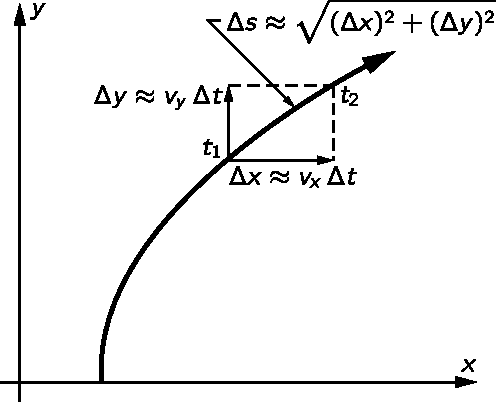
\includegraphics[width=5cm]{Chapter8/物体二维运动的描述和它的速度的计算}
        \caption{物体二维运动的描述和它的速度的计算}
        \label{figure:物体二维运动的描述和它的速度的计算}
    \end{minipage}
    \begin{minipage}[t]{0.45\textwidth}
        \centering
        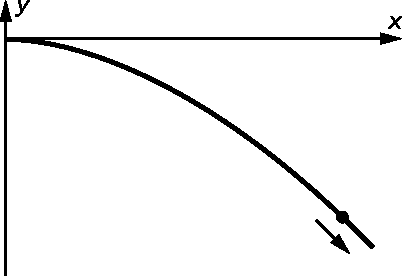
\includegraphics[width=5cm]{Chapter8/具有水平初速的落体所描述的抛物线}    
        \caption{具有水平初速的落体所描述的抛物线}
        \label{figure:具有水平初速的落体所描述的抛物线}
    \end{minipage}
\end{figure}

让我们考虑一个在平面内复合运动的很好的例子。取一个在水平方向以匀速$u$运动同时在垂直向下的方向又以匀加速度($-g$)运动的球;它的运动是怎样的呢?我们可以说$dx/dt=v_x=u$。因为速度$v_x$是常数,故
\begin{equation}
\label{Eq:I:8:17}
x=ut,
\end{equation}
而由于向下的加速度$-g$是常数,球体落下的距离$y$可写为
\begin{equation}
\label{Eq:I:8:18}
y=-\tfrac{1}{2}gt^2.
\end{equation}
路程的曲线,即$y$与$x$之间的联系是怎样的呢?因为$t=x/u$,我们可以从方程(\ref{Eq:I:8:18})消去$t$。把它代入以后,求得
\begin{equation}
    \label{Eq:I:8:19}
    y=-\frac{g}{2u^2}x^2.
\end{equation}
这个$y$与$x$之间的关系式可视为正在运动的小球的路径的方程。当画出这个方程的图形时,我们得到一条称为抛物线的曲线;向任何方向射出的自由落体都将以抛物线的形式行进,如图8.4所示。 